\begin{slikaDesno}{fig/z_stab.pdf}
    \PID У блок диjаграму дискретног система са слике позната jе преносна функциjа
    $G(z) = \frac{1}{z - 2}$. Израчунати појачање $A$ идеалног појачавача тако да је 
    дати систем представљен дијаграмом, $H(z) = \dfrac{Y(z)}{X(z)}$ асимптотски стабилан
\end{slikaDesno}

\RESENJE
На основу датог блок дијаграма, улаз у систем $G(z)$ је $X(z) - AY(z)$ па се на основу карактеристике тог система има 
\begin{eqnarray}
    Y(z) = G(z) \left( X(z) - AY(z) \right) \Rightarrow Y(z) = \underbrace{\dfrac{G(z)}{ 1 + AG(z) }}_{H(z)} X(z) 
\end{eqnarray}
Добијена укупна функција преноса целог система се онда може поједноставити заменом датог облика $G(z)$ као 
\begin{eqnarray}
    H(z) = \dfrac{G(z)}{ 1 + AG(z) }
         = \dfrac{\dfrac{1}{z - 2}}{1 + \dfrac{A}{z - 2}} 
         = \dfrac{1}{z - 2 + A}
\end{eqnarray}
Стабилност дискретног система може се испитати провером структуре његових полова. 
Конкретно, област стабилности дискретних система јесте јединична кружница у $z$-равни.
Уколико је једини пол посматраног система унутар те кружнице, систем је стабилан. У овом случају систем тај један пол
се налази као корен полинома у имениоцу, као $z_{\rm p} - 2 + A = 0$, односно 
\begin{equation}
    z_{\rm p} = 2-A.
\end{equation} У анализи дискретних система, стабилност система са једним полом зависи
од његовог модула, односно од $|z_{\rm p}| = 2-A$. Дијаграм ове зависности приказан је на слици. 
\begin{figure}[ht!]
    \centering
    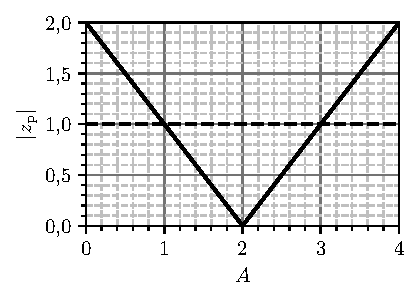
\includegraphics{fig/z_mod.pdf}
    \caption{Зависност $|z_{p}|(A)$, критична вредност $z_{\rm p} = 1$ уцртана је испрекидано }
\end{figure}

Коначно, скуп свих вредности $A$ за које је овај систем асимптотски стабилан је скуп решења неједначине $|z_{\rm p}|<1$, односно 
$1 < A < 3$. 
